\chapter{二分图中的极大二分团枚举问题}
\label{ch:intro}

二分图是图论中一种基本结构,被广泛应用于社交网络分析、推荐系统、生物信息学等领域。在二分图中,极大二分团是特殊的子图,用于描述不同群体之间的连接关系,具有重要的研究价值和应用潜力。极大二分团枚举问题在数据挖掘和图论领域中扮演着重要角色,帮助我们理解图的结构和特征,并挖掘有用的信息。例如,在电子商务中,极大二分团可以描述同时购买某批商品的用户群体,通过枚举极大二分团,可以提高对刷单行为的检测率。然而,随着二分图规模的增大,极大二分团的数量也不断增加,如何高效地进行枚举成为一个严峻挑战。本章首先概述二分图中极大二分团枚举问题的定义,随后介绍基于集合枚举树进行极大二分团枚举的基本方法,最后讨论现有方法存在的问题和挑战。

% 二分图是图论中的一种基本结构,广泛应用于许多领域,如社交网络分析、推荐系统、生物信息学等。在二分图中,极大二分团是一种特殊的子图,用来最大程度地描述两个不同群体间的连接关系,具有重要的研究价值和应用潜力。二分图中的极大二分团枚举问题在数据挖掘领域和图论领域中扮演着重要的角色,因为他可以帮助我们更好的理解图的结构和特征,进而从中挖掘有用的信息。例如,在电子商务场景中,极大二分团描述同一批用户同时购买了同一批商品。通过对极大二分团的枚举,便于找到可以交易,提升对刷单行为的检出率。随着大数据时代的到来,二分图的规模不断扩大,极大二分团的数量不断增多,在短时间内完成极大二分团枚举的计算成为了一个严峻的挑战。本章给出了二分图中的极大二分团枚举问题的概述,包括问题定义以及现有方法存在的问题与挑战。

\section{问题定义}

在问题定义之前,我们首先介绍图论领域的一些基础概念,并提供了随后频繁使用的符号及其含义,如表~\ref{tab:definition}所示。

\begin{longtable}[htbp]{|c|p{12cm}|}
    \caption{本文使用的符号及含义}
    \label{tab:definition} \\
    
    \hline
    符号 & 含义 \\ \hline
    \endfirsthead
    
    \hline
    符号 & 含义 \\ \hline
    \endhead
    
    \hline
    \multicolumn{2}{r}{续下页} \\
    \endfoot
    
    \hline
    \endlastfoot
    
    $G(U,V,E)$ & 一个无向二分图 $G$,其中 $U$ 和 $V$ 是两个不相交的顶点集合,$E$ 是二分图的边集合且 $E \subseteq U \times V$。 \\ \hline
    $u,v$ & 表示二分图 $G$ 中的顶点。其中顶点 $u$ 属于集合 $U$,顶点 $v$ 属于集合 $V$。 \\ \hline
    $N(v)$ & 表示顶点 $v$ 的邻居顶点集合,即 $N(v) = \{u \,|\, (u,v) \in E\}$。 \\ \hline
    $N_2(v)$ & 表示顶点 $v$ 的二跳邻居顶点集合,即 $N_2(v) = \bigcup_{u \in N(v)} N(u) - \{v\}$。 \\ \hline
    $\Delta(v)$ & 表示顶点 $v$ 的度数,即 $\Delta(v) = |N(v)|$。 \\ \hline
    $\Gamma(X)$ & 表示顶点集 $X$ 内顶点的共同邻居,即 $\Gamma(X) = \bigcap_{v \in X} N(v)$。 \\ \hline
    $\Delta(X)$ & 表示顶点集 $X$ 内顶点的最大度数,即 $\Delta(X) = \max_{u \in X} |N(u)|$。 \\ \hline
    $\Delta_2(X)$ & 表示顶点集 $X$ 内顶点的最大二跳度数,即 $\Delta_2(X) = \max_{u \in X} |N_2(u)|$。 \\ \hline
    $X_v^+, X_v^-$ & 表示顶点集 $X$ 根据顶点 $v$ 划分成的两个子集。给定一个顶点顺序,$X_v^+$ 包含所有顶点比 $v$ 更大的顶点(顺序在 $v$ 之后的顶点),即顶点$v$的尾部顶点;$X_v^-$ 包含包括 $v$ 顶点在内的所有顶点比 $v$ 更小的顶点(顺序在 $v$ 之前的顶点),即顶点$v$的头部顶点。 \\ \hline
    $L,R,C$ & $L$, $R$ 和 $C$ 指三个两两不相交的顶点集,其中 $L$ 是集合 $U$ 的子集,$R$ 和 $C$ 是集合$V$ 的子集。$L,R$ 和 $C$ 共同构成一个枚举树节点,其中 $(L,R)$ 表示枚举树节点对应的二分团,$C$ 表示用于生成新枚举树节点的候选顶点。对于二分团 $(L,R)$,$L$ 和 $R$ 分别表示二分团的左部顶点集和右部顶点集。 \\ \hline
    $N_L(v)$ & 表示顶点 $v$ 的局部邻居。对于对应二分团 $(L,R)$ 的枚举树节点,$N_L(v) = L \cap N(v)$。 \\ \hline
    $\vec{v}$ & 对于一个枚举树节点,$\vec{v}$ 表示用于生成该枚举树节点的候选顶点。 \\ \hline
    $\alpha, \delta, \beta$ & 对于一棵极大二分团枚举树,$\alpha$ 表示枚举树中产生的极大二分团的数量,$\delta$ 表示枚举树中产生的其他二分团的数量,$\beta$ 表示枚举树中二分团的总数量。可知 $\beta = \alpha + \delta$。 \\ \hline
\end{longtable}

  二分图中的极大二分团枚举问题是在一个无向二分图$G(U,V,E)$中的子图挖掘问题。随后,我们正式定义二分团、极大二分团以及极大二分团枚举问题。

\begin{definition}
  \textbf{(二分团)} 二分团(biclique)是二分图$G(U,V,E)$中的稠密二分子图$(L,R,E')$。其中$L\subseteq U$, $R\subseteq V$, $E' = L \times R \subseteq E$。为了方便,下文中我们直接用顶点集对$(L,R)$表示二分团。
\end{definition}

\begin{definition}
  \textbf{(极大二分团)} 极大二分团(maximal biclique)是二分图$G$中的一个二分团,且该二分团不能再添加其他顶点使其成为更大的二分团。
  \label{def:mb}
\end{definition}

\begin{definition}
  \textbf{(极大二分团枚举问题)} 本文所研究的极大二分团枚举问题(maximal biclique enumeration, MBE)的目标是无重复、无遗漏地枚举二分图中的全部极大二分团。
\end{definition}

\begin{figure} [ht]
  \vspace{0.2 in}
  \centering
  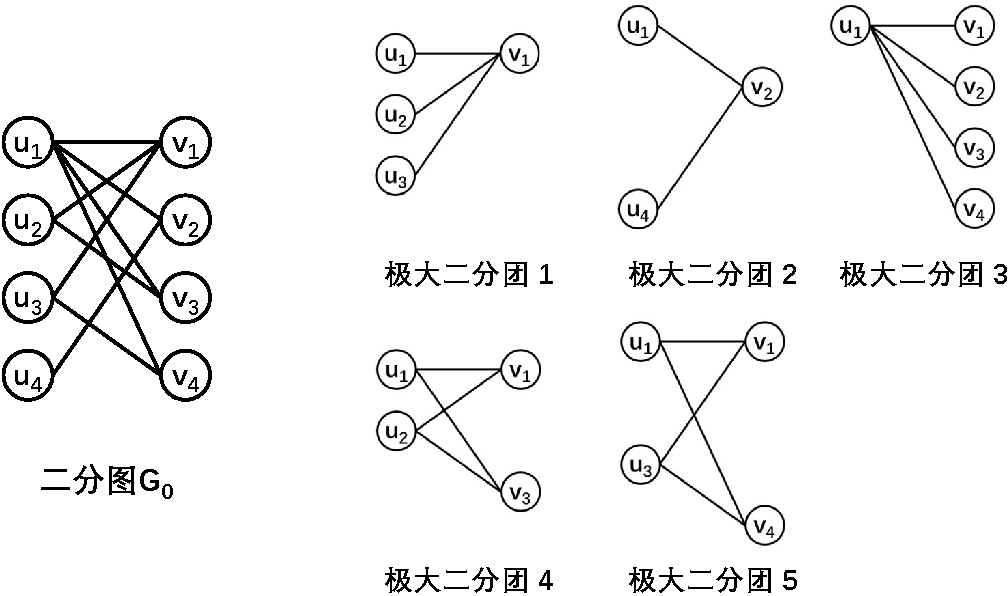
\includegraphics[width=0.7\linewidth]{eg_definition}
  \vspace{0.1 in}
  \caption{二分图中的极大二分团枚举问题示例}
  \label{fig:eg_definition}
\end{figure}

\begin{example}
  图~\ref{fig:eg_definition}给出了一个二分图中的极大二分团枚举问题的示例。其中左图是一个具有8个顶点,9条边的二分图$G_0$,右图展示了二分图中的全部极大二分团,共5个。
  
\end{example}

\section{基于集合枚举树的极大二分团枚举方法}
\label{sec:se}


集合枚举树是解决集合问题的强大工具,在主流的极大二分团枚举算法中扮演着重要角色。本节将详细介绍集合枚举树,并介绍基于该树的极大二分团枚举算法,并分析其算法复杂度。


\begin{figure} [ht]
  \vspace{0.1 in}
  \centering
  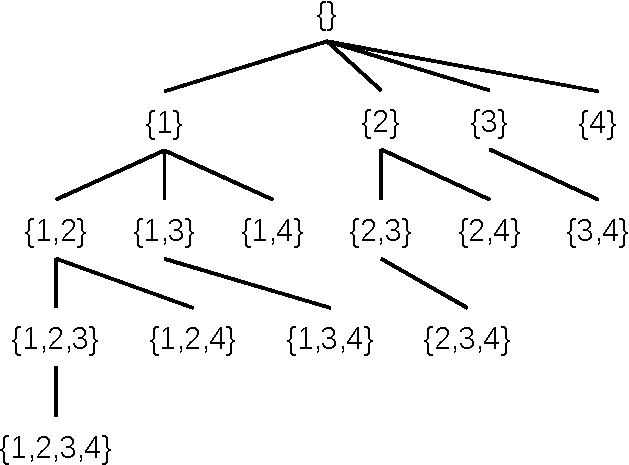
\includegraphics[width=0.5\linewidth]{se_naive}
  \vspace{0.05 in}
  \caption{对于集合$P\{1,2,3,4\}$的集合枚举树}
  \label{fig:se_naive}
\end{figure}


% 集合枚举树(set enumeration tree, SE-tree)是一种用于有序地枚举特定集合全部子集的数据结构~\cite{SEtree92},即枚举该集合的幂集。如果问题的搜索空间是特定集合幂集的一个子集,集合枚举树可引导一种完整且无冗余的搜索技术。具体地,如图~\ref{fig:se_naive}所示,在集合枚举树中,树的根节点表示空集。每个节点对应一个子集,节点的子节点表示在该子集的基础上添加一个新元素所得到的子集。对于二分图中的极大二分团枚举问题而言,每个二分团的$R$集合是二分图中$V$集合中的一个独特的子集,因此,可以引入集合枚举树进行问题求解。

\subsection{集合枚举树介绍}
\label{subsec:se}


\textbf{集合枚举树}(set enumeration tree, SE-tree)是一种用于有序地枚举特定集合全部子集的数据结构,即枚举该集合的幂集~\cite{SEtree92}。它为解决搜索空间为特定集合幂集的子集的问题提供了一种完整且无冗余的搜索技术。具体而言,集合枚举树如图~\ref{fig:se_naive} 所示,根节点表示空集,每个节点对应一个子集,其子节点代表在该子集基础上添加一个新元素所得到的子集。对于二分图中的极大二分团枚举问题而言,每个二分团的集合$R$即为二分图中集合$V$的一个独特子集。因此,通过引入集合枚举树可以有效地求解该问题。

对于应用于极大二分团枚举问题的集合枚举树,我们从以下三个角度对其进行了规范化描述:

\begin{itemize}
  \item 节点结构:每个树节点为一个三元组$(L,R,C)$。在一个二分图$G(U,V,E)$,集合$L$是集合$U$的子集,集合$R$和集合$C$是集合$V$的两个不相交子集。集合$L$和$R$构成一个二分团,其中集合$L$包含左部顶点,集合$R$包含右部顶点。集合$C$包含用于扩展集合$R$的候选顶点。
  \item 节点生成:枚举树从根节点$(U,\emptyset,V)$ 开始遍历。对于当前节点$(L,R,C)$,枚举树按顺序访问$C$集合中的每个候选顶点$v'$以生成一个新的节点$(L',R',C')$。集合$L'$包含集合$L$和集合$N(v')$中的共同顶点。集合$R'$包含集合$R$中的顶点、顶点$v'$以及集合$C$中与集合$L'$内顶点均相连且未被访问的顶点。集合$C'$包含集合$C$中与集合$L'$内顶点部分相连的且未被访问的顶点。
  \item 节点检查:当且仅当集合$L'$的共同邻居等于集合$R'$, 即$\Gamma(L')=R'$时,节点$(L',R',C')$通过节点检查,输出一个极大二分团。
\end{itemize}

此外,一些研究~\cite{iMBEA14,ooMBE22}在每个枚举节点中额外引入集合$Q$作为辅助节点检查的工具,构成四元组$(L,R,C,Q)$。集合$Q$于存储已访问的候选顶点,以帮助确定是否存在非极大二分团。具体而言,当集合$Q$中存在一个顶点$v_q$,并且它的邻居包含了集合$L$中的所有顶点时,根据定义~\ref{def:mb}我们可以推断当前节点对应的二分团$(L,R)$可以添加顶点$v_q$构成新的二分团,从而判定当前节点对应一个非极大二分团。然而,使用集合$Q$需要额外的存储和计算开销。幸运的是,我们观察到可以通过访问$L$中的任意顶点$u_l$的邻居$N(u_l)$来高效地替代集合$Q$的作用。具体而言,当集合$N(u_l)$中存在一个不在不在$R$集合中的顶点$v^*$,并且它的邻居包含了集合$L$中的所有顶点时,我们可以推断当前节点对应的二分团$(L,R)$可以添加顶点$v^*$构成新的二分团,从而判定当前节点对应一个非极大二分团。因此,在枚举树的介绍和相关算法中,我们不再引入集合$Q$。

\subsection{基于集合枚举树的极大二分团枚举算法}
根据前一节对应用于极大二分团枚举问题的集合枚举树的描述,我们给出了基于集合枚举树的极大二分团枚举的算法。

\begin{algorithm}[H]
    \begin{algorithmic}[1]
        \normalsize
        \REQUIRE 二分图 $G(U,V,E)$
        \ENSURE 所有极大二分团
        
        \renewcommand{\algorithmicwhile}{\textbf{procedure}}
        \renewcommand{\algorithmicdo}{\textbf{:}}


        \STATE \textsf{biclique\_search\_basic}$(U,\emptyset,V)$;
        \WHILE{\textsf{biclique\_search\_basic}$(L,R,C)$}
        \renewcommand{\algorithmicdo}{\textbf{do}}
          \FOR{$v' \in C$}
            \STATE $L' \leftarrow L \cap N(v')$; $R'\leftarrow R$; $C' \leftarrow \emptyset$;
            \FOR{$v_c \in C$}
              \IF{$L' \cap N(v_c) = L'$}
                \STATE $R' \leftarrow R' \cup \{v_c\}$;
              \ELSIF{$L' \cap N(v_c) \neq \emptyset$}
                \STATE $C' \leftarrow C' \cup \{v_c\}$;
              \ENDIF
            \ENDFOR
            \IF{$\Gamma(L') = R'$}
              \STATE 输出极大二分团$(L', R')$;
              \STATE \textsf{biclique\_search\_basic}$(L',R',C')$;
            \ENDIF
            \STATE $C \leftarrow C \setminus \{v'\}; $
          \ENDFOR

        \ENDWHILE

    \end{algorithmic}
    \caption{基于集合枚举树的MBE算法}
    \label{alg:se_mbe}
\end{algorithm}

算法~\ref{alg:se_mbe}总结了基于集合枚举树的极大二分团枚举算法的基本枚举过程。该算法从根节点$(U,\emptyset,V)$开始,并递归地调用\textsf{biclique\_search\_basic}过程 (第1行)。过程\textsf{biclique\_search\_basic}接收一个枚举树节点作为输入,即集合$L$,$R$和$C$ (第2行)。在处理当前枚举节点时,该过程会逐个遍历$C$中的顶点$v'$ (第3行),然后根据集合枚举树的节点生成规则生成新节点$(L',R',C')$ (第4-11行)。随后,过程按照节点检查规则对新生成的节点$(L',R',C')$进行检查 (第12行)。如果该节点对应一个极大二分团,则输出该二分团 (第13行),并递归地调用过程\textsf{biclique\_search\_basic}以节点$(L',R',C')$为根节点继续探索子枚举树 (第14行)。为保证$C$中的顶点都未被访问,过程会及时从$C$中移除已访问的顶点$v'$ (第16行)。我们用下面的例子对该算法进行说明。


\begin{figure} [ht]
  \vspace{0.1 in}
  \centering
  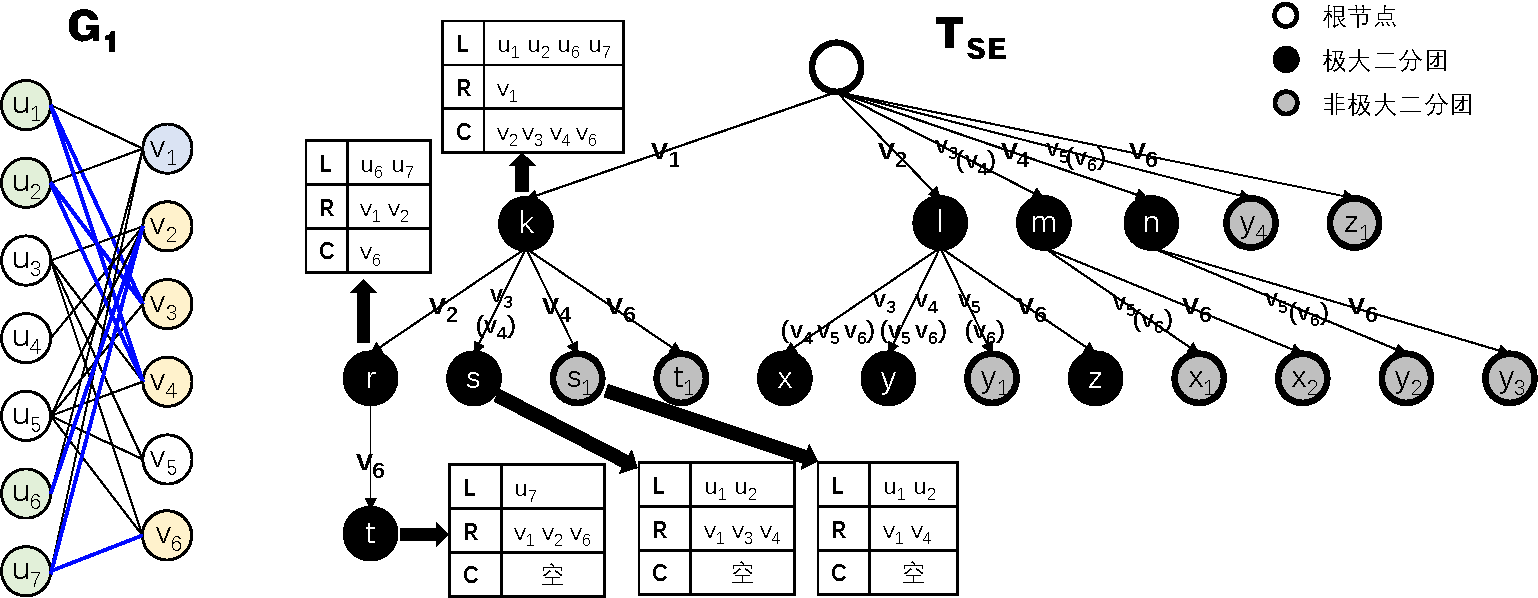
\includegraphics[width=0.9\linewidth]{se_mbea}
  \vspace{0.05 in}
  \caption{算法~\ref{alg:se_mbe}在二分图$G_1$上的集合枚举树}
  \label{fig:se_mbea}
\end{figure}

\begin{example}
  \label{example:se}
  图~\ref{fig:se_mbea}展示了算法~\ref{alg:se_mbe}在二分图$G_1$上的集合枚举树$T_{SE}$。
  \footnote{为了方便比较,整个文中具有相同字母标识的节点在枚举树中共享相同的集合$L$,只有没有下标的节点会输出极大二分团。例如,节点$s$和节点$s_1$具有相同的$L$集合,但只有节点$s$会输出一个极大二分团。我们使用集合的下标来表示该集合隶属于哪个节点。例如$L_s$表示节点$s$的集合$L$。 
}
我们从根节点开始,通过深度优先搜索逐个遍历候选顶点,递归地搜索子空间。首先,我们通过遍历顶点$v_1$生成节点$k$。按照算法~\ref{alg:se_mbe}中第4-11行的计算方法,我们可以计算得到$L_k=\{u_1, u_2, u_6, u_7\}$, $R_k=\{v_1\}$,$C_k=\{v_2,v_3,v_4,v_6\}$。根据节点检查规则,因为$\Gamma(L_{k}) = \{v_1\} = R_{k}$,所以节点$k$输出一个极大二分团并继续探索以节点$k$为根节点的子枚举树。为便于观察,我们在图$G_1$中标记了节点$k$中的顶点,并标出了集合$L_k$与集合$C_k$之间的边。

接下来,节点$k$遍历顶点$v_2$生成节点$r$。同理,我们可以计算得到$L_{r} = N(v_2) \cap L_{k} 
= \{u_3, u_4, u_5, u_6, u_7\} \cap \{u_1, u_2, u_6, u_7\} = \{u_6, u_7\}$, $R_{r} = R_{k} \cup (C_{k} \cap \Gamma(L_{r})) = \{v_1\} \cup (\{v_2, v_3, v_4, v_5\} \cap \{v_1, v_2\}) = \{v_1, v_2\}$。集合$C_{r}$中仅包含顶点 $v_6$,因为顶点$v_3$, $v_4$和 $v_5$不与集合$L$中的任何顶点相连。

继续这个过程,我们可以计算得到节点$s$以及节点$s_1$。节点$s$对应二分团$(\{u_1, u_2\}$, $\{v_1, v_3, v_4\})$,节点$s_1$对应二分团 $(\{u_1, u_2\}, \{v_1, v_4\})$。根据节点检查规则,因为$\Gamma(L_{s_1}) = \{v_1, v_3, v_4\} \neq R_{s_1} = \{v_1, v_4\}$,所以节点$s_1$对应一个非极大二分团。具体地,与节点$s$相比,节点$s_1$不能用$v_3$来扩展该节点中的集合$R_{s_1}$。这是因为在生成节点$s_1$时,根据深度优先搜索的规则,顶点$v_3$已被访问并用于生成节点$s$。因此,在节点检查之后,我们删除了节点$s_1$。同理,其他节点可以类似地生成。

\end{example}

在算法~\ref{alg:se_mbe}的基础上,现有的基于枚举树的极大二分团枚举算法的优化方法主要包括变节点候选顶点的遍历顺序~\cite{minel06,iMBEA14,PMBE20,ooMBE22}、设计剪枝方法以提前裁剪产生非极大二分团的节点~\cite{iMBEA14,PMBE20,ooMBE22},以及并行优化~\cite{mapreduceMBE16,parMBE18}。在~\ref{sec:opt}节中,我们将对上述优化方法进行详细说明,并介绍它们在实际应用中的效果。

\subsection{算法复杂度分析}
\label{subsec:baseline_analysis}

本节从时间复杂度和空间复杂度两个方面对算法~\ref{alg:se_mbe}进行分析。

\textbf{时间复杂度:} 我们首先分析枚举树中每个节点的计算时间,随后分析枚举树中的枚举节点数量,最终得到算法~\ref{alg:se_mbe}的时间复杂度。平均而言,对于每个节点$(L',R',C')$的计算包括节点生成(第4-11行)和节点检查(第12行)两个部分。由于集合$C$中最多包含$|V|$个顶点,且每个顶点的集合求交操作需要$\BigO{\Delta(V)}$的时间,因此节点生成过程的时间复杂度为$\BigO{|V|\Delta(V)}$。而节点检查过程中,我们可以通过只访问二分图中的每条边一次来获取$\Gamma(L')$的值,因此节点检查的时间复杂度为$\BigO{|E|}$(或$\BigO{|V|\Delta_{avg}(V)}$)。综上,每个节点的计算时间为$\BigO{|V|\Delta(V)}$。为了量化算法的计算时间,我们用$\beta$来表示枚举树中节点的数量。最终,算法的时间复杂度为$\BigO{|V|\Delta(V)\beta}$。

\textbf{空间复杂度:} 由于算法~\ref{alg:se_mbe}按照深度优先的方式进行搜索,我们可以对枚举树中每个节点占用的空间进行分析,并结合枚举树的高度以及输入二分图所占用的空间,得到算法的空间复杂度。对于每个节点$(L',R',C')$,集合$L'$最多包含$\Delta(V)$个顶点,集合$R'$和$C'$最多包含$|V|$个顶点。在二分图中,集合$V$内顶点的数量通常远高于任何单个顶点的度数,因此每个节点的空间开销为$\BigO{\Delta(V)+|V|}=\BigO{|V|}$。在递归过程中,节点的集合$L$内的顶点数量不断减少,因此我们可以确定枚举树的高度为$\BigO{\Delta(V)}$。考虑到二分图$G(U,V,E)$需要占用$\BigO{|U|+|V|+|E|}=\BigO{|E|}$的空间,最终算法的空间复杂度为$\BigO{|E|+|V|\Delta(V)}$。

\section{存在的问题与挑战}

尽管在极大二分团枚举领域已经有很多出色的工作,但是在处理大规模二分图时,已有方法的计算性能仍然有很大的提升空间。本节将指出现有基于集合枚举树的枚举方法所面临的三个共性问题,并介绍解决这些问题所面临的具体挑战。

\subsection{搜索空间大,剪枝方法欠佳}

极大二分团枚举问题具有搜索空间大的特点。常见的图算法,如深度优先搜索~\cite{wiki-dfs}、广度优先搜索~\cite{wiki-bfs}、最小生成树~\cite{wiki-mst}、最短路径等算法~\cite{wiki-sssp},其搜索空间随着图的规模线性增长。常见的图模式挖掘算法的目标子图往往只包含少量顶点~\cite{g2miner22,decomine22,khuzdul23,gamma23},例如三角计数问题中目标子图仅包含3个顶点~\cite{triangle18}。相比之下,极大二分团枚举问题的搜索空间更大,因为它随着二分图中顶点数量的指数级增长,并且目标子图(即极大二分团)中的顶点数量相对较多。为了应对搜索空间巨大的挑战,研究人员提出了各种优化技术,旨在减少搜索空间中产生非极大二分团的无效枚举节点,进而减少枚举时间。然而,由于搜索空间的规模庞大,现有的优化方法往往难以完全覆盖所有无效节点。具体而言,通过~\ref{subsec:ambea_exp_overall}节的实验,我们观察到现有的最新算法ooMBEA在Github数据集上需要检查并消除比极大二分团数量多26倍的产生非极大二分团的无效枚举节点。这些无效枚举节点带来大量的节点检查开销,严重降低了计算性能。因此,如何设计高效的剪枝方法来裁剪巨大搜索空间仍然是一个关键的挑战。

% 首先,极大二分团枚举问题面临的搜索空间巨大的问题。根据枚举树的定义,在二分图$G(U,V,E)$中,极大二分团枚举问题的搜索空间是$V$集合的幂集。这意味着随着二分图顶点数量的增加,求解这个问题的困难程度呈指数级增长~\cite{MICA04}。为了应对这个挑战,研究者们提出了多种搜索空间优化方法,旨在减少产生非极大二分团的无效枚举节点。然而,由于搜索空间的规模庞大,现有的优化方法往往难以完全覆盖所有无效节点。具体而言,通过~\ref{subsec:ambea_exp_overall}节的实验,我们观察到现有的最新算法ooMBEA在Github数据集上需要检查并消除比极大二分团数量多26倍的产生非极大二分团的枚举节点。这些枚举节点带来大量的节点检查开销,严重降低了计算性能。因此,如何设计高效的剪枝方法来裁剪巨大的搜索空间是一个重要挑战。

\subsection{计算不规则,单一结构低效}

极大二分团枚举问题具有计算不规则的特点。与其他图计算问题类似,在真实世界中,二分图的顶点邻居数量存在较大差异,导致每次计算涉及的顶点数量不同,即计算不规则~\cite{Irregularity12}。为了高效地解决这类问题,研究者们提出了多种存储结构来表示图的邻接关系。常用的存储结构包括位图~\cite{lcm04,lcmmbc07,FCA15,FCA21,FCA22}、邻接表~\cite{iMBEA14,PMBE20,ooMBE22}和哈希表~\cite{parMBE18}。不同的存储结构适用于不同场景。
例如,位图结构采用位运算,具有高效的计算能力,但在稀疏图场景下会占用更多的存储资源,因此适用于稠密小图;邻接表精确地存储每个顶点的邻居信息,在处理稀疏大图时占用较少的内存,但计算过程需要执行大量的比较运算,其执行时间与顶点个数成正比,会导致计算相对低效,因此适用于稀疏大图;哈希表具有灵活性和便于快速查找的特点,可以快速判断任意两个顶点之间的连接关系,但相比邻接表,它需要更多的存储空间并且访问方式更为随机。然而,目前的研究往往采用固定的数据结构来存储顶点的邻居信息,未能充分发挥不同数据结构的优势。因此,在枚举过程中如何动态选择合适的存储结构,发挥计算潜力,是一个关键挑战。


% 与其他图计算问题类似,极大二分团枚举主要涉及集合运算。由于真实世界中二分图中顶点的邻居数量存在较大差异,因此集合运算的执行时间也会有所不同,导致计算不规则的情况~\cite{Irregularity12}。集合运算的执行方式与二分图顶点邻居的存储结构有关,常用的存储结构包括位图~\cite{lcm04,lcmmbc07,FCA15,FCA21,FCA22}、邻接表~\cite{iMBEA14,PMBE20,ooMBE22}和哈希表~\cite{parMBE18}。不同的存储结构适用于不同的场景。例如,位图结构可以通过位运算快速实现集合计算,但在稀疏图的情况下会占用较多存储资源,适用于稠密小图;而邻接表可以精确地存储每个顶点,占用较少内存,但计算过程涉及大量比较运算,执行时间与顶点个数成正比,适用于稀疏大图;哈希表可以快速判断任意两个顶点之间的连接关系,灵活适用的场景多样,但相比邻接表需要更多存储空间和随机访问。然而,现有研究工作往往采用固定的数据结构来存储顶点的邻居信息,并进行集合操作,未能充分发挥不同数据结构的优势。因此,在枚举过程中如何动态选择数据结构,发挥计算潜力,是一个关键挑战。

% 其次,现有的方法往往采用单一的数据结构。在早期的工作~\cite{lcmmbc07}以及闭频繁项挖掘~\cite{lcm04}和形式概念分析~\cite{FCA15,FCA21,FCA22}等相关研究中,为了提高集合操作的计算效率,采用了位图数据结构。位图通过使用二进制位来表示集合中的元素,实现了高效的位操作。然而,随着二分图规模的增大,由于二分图的稀疏性,位图会占用大量存储空间,因此这些方法无法应用于大规模二分图。目前主流的极大二分团枚举工作通常采用邻接表作为数据结构~\cite{iMBEA14,PMBE20,ooMBE22}。邻接表数据结构将每个节点的邻居节点列表存储在一个链表中,适用于表示稀疏图。邻接表具有存储空间小、获取顶点邻居操作简单等优点。然而,与位图相比,基于邻接表的集合操作需要更长的执行时间。还有一些工作采用了哈希表数据结构~\cite{parMBE18},通过使用哈希函数将关键字映射到索引位置,实现快速查找操作。然而,随着二分图规模的增加,哈希表会引入大量的随机访问和存储开销,从而降低计算性能。因此,如何根据不同情况灵活选择适合的数据结构以提高计算性能是一个重要挑战。

\subsection{负载不均匀,并行扩展性差}

极大二分团枚举问题具有负载不均匀的特点,限制了问题的并行扩展能力。为了进一步提高问题求解的效率,研究人员尝试设计并行算法来处理极大二分团枚举问题~\cite{mapreduceMBE16, MBEHe18, parMBE18}。这些算法将整个集合枚举树分解成多个子枚举树,然后利用分布式系统或多核CPU的大量计算资源来并行处理这些子树。然而,由于不同子枚举树的极大二分团的大小不同,导致计算负载之间存在较大差异。因此,即使有大量计算资源可用,计算任务的执行时间仍然受限于最耗时的负载。GPU作为一种专门用于并行计算的硬件设备,由于其内部拥有大量的计算单元,非常适合处理并行任务。然而,由于GPU和CPU在体系结构、内存层次结构以及编程模型等方面存在较大差异,现有的极大二分团枚举算法无法直接迁移到GPU系统中。此外,极大二分团枚举问题的不规则计算模式和不均匀负载进一步增加了在GPU上设计并行算法的难度。因此,如何实现负载均衡并突破现有算法在并行能力方面的限制,设计基于GPU的并行极大二分团枚举方法是一个重要挑战。


% 最后,现有方法的性能受到其并行扩展能力的限制。尽管已有研究探索了基于分布式计算和多核CPU计算的并行枚举算法~\cite{mapreduceMBE16,parMBE18},但这些算法仅适用于CPU的并行计算。然而,在真实系统中,CPU数量通常不会超过100个,因此这些并行算法的性能受到CPU数量的限制。尽管GPU由于其大量的计算核心而在并行算法中广泛应用,但现有基于CPU的枚举算法无法直接迁移到GPU系统中。这是因为GPU和CPU在体系结构、内存层次结构以及编程模型等方面存在较大差异。因此,如何突破现有算法在并行能力方面的限制,设计基于GPU的并行计算方法是一个重要挑战。

\section{本章小结}

本章首先介绍了二分图中的极大二分团枚举问题的定义。随后结合伪代码以及实例介绍了基于集合枚举树的极大二分团枚举基本方法,并对算法复杂度进行分析。最后针对极大二分团枚举问题的搜索空间大、计算不规则以及负载不均匀三个特点,指出现有方法存在的问题与挑战。